\documentclass[10pt,twocolumn,letterpaper]{article}

\usepackage{cvpr}
\usepackage{times}
\usepackage{epsfig}
\usepackage{graphicx}
\usepackage{amsmath}
\usepackage{amssymb}

% Include other packages here, before hyperref.

% If you comment hyperref and then uncomment it, you should delete
% egpaper.aux before re-running latex.  (Or just hit 'q' on the first latex
% run, let it finish, and you should be clear).
\usepackage[pagebackref=true,breaklinks=true,letterpaper=true,colorlinks,bookmarks=false]{hyperref}

 \cvprfinalcopy % *** Uncomment this line for the final submission

\def\cvprPaperID{****} % *** Enter the CVPR Paper ID here
\def\httilde{\mbox{\tt\raisebox{-.5ex}{\symbol{126}}}}

% Pages are numbered in submission mode, and unnumbered in camera-ready
\ifcvprfinal\pagestyle{empty}\fi
\begin{document}

%%%%%%%%% TITLE
\title{Improving Millimeter Wave Radar Perception with Deep Learning}

\author{Junfeng Guan \hspace{2cm} Sohrab Madani\\
ECE 544 Project Reportl\\
{\tt\small jguan8@illinois.edu  \hspace{2cm} smadani2@illinois.edu}
% For a paper whose authors are all at the same institution,
% omit the following lines up until the closing ``}''.
% Additional authors and addresses can be added with ``\and'',
% just like the second author.
% To save space, use either the email address or home page, not both
}

\maketitle
%\thispagestyle{empty}

%%%%%%%%% BODY TEXT
%section 
\section{Introduction and Project Descriptions} \label{introduction}

%Describe the proposed problem, give background information via a thorough literature review. If you are proposing a new method, you should also clearly state the gap between the current literature and your work (e.g., what new contribution(s) does your method make?)

Since the past few years, AI-Powered autonomy revolution in the automotive industry has attracted great attention worldwide. It is believed that in the not-too-distant future, fullyautonomous vehicles will be the norm rather than the exception, redefining mobility in our daily lives. With deep learning widely applied on sensor data, self-driving cars are able to localize and map objects, understand the environment, and make correct decisions. As the most fundamental task, previous works have demonstrated accurate object detection and classification, but they are limited to data obtained from LiDARs and cameras. These optical sensors have high imaging resolution, but they naturally fail in low visibility conditions such as fog, rain, and snow, because light beams are narrower than water droplets and snowflakes.~\cite{snow} This fundamental limitation of optical sensors is one of the major roadblocks to achieving the 5th SAE level of full automation. ~\cite{SAE} On the contrary, Radar wave propagates through small particles and can provide an alternate imaging solution in such inclement weather. Besides, radar can also directly measure the velocity of vehicles based on the doppler shift of the reflected signal instead of going through cluster tracking among frames like LiDAR. With the additional realtime speed information, AI can potentially have a better perception than human drivers.

Although the low resolution of traditional automotive radar overshadows its advantages, the advent of Millimeter-wave (mmWave) technology makes it possible to have a reliable 3D imaging system in inclement weather with relatively higher resolution. Along with good propagation characteristics, mmWave also provides much wider bandwidth and enables miniature-sized large-aperture antenna arrays, which improve distance and angle measurement respectively. Previous work has demonstrates sub-centimeter level imaging resolution for short range objects ~\cite{mmWave_SAR}, but the fundamental difference in wavelength between radar (5 mm) and LiDAR (905 nm) cannot be easily overcome. Moreover, radar images are not as readable to non-experts. Therefore, in order to convince the automotive industry and general public that mmWave is a reliable imaging solution for autonomous driving, we should try to generate radar images targeting the resolution comparable to LiDAR, and make them more perceptually intuitive to people. 

In this project, we propose to develop high-resolution and reliable imaging techniques for self-driving cars with mmWave radar. Specifically training neural networks to enhance the low-resolution and unreadable radar images to be similar to the LiDAR point cloud, which has been extensively and successfully used for self-driving perception. Eventually enable various crucial vision applications for autonomous vehicles like lane detection, image mapping, localization, and object identification with mmWave radar data only. To do this, we have to overcome challenges analyzed in the following section \ref{challenges}.
 
 % Jayden

%section
\section{Challenges}
\subsection{Radar Imaging Primer}
Radar generates images of objects by localizing the cluster of point reflectors that forms the object. 3D space imaging requires mapping point reflectors to voxels in a spherical coordinates with its distance, azimuth angle, and elevation angle. Distance is measured through to round-trip Time-of-Flight (ToF) of reflected radar signal, while azimuth and elevation angles can be either obtained by the beam steering angle of phased array antennas or be estimated with Direction-of-Arrival (DoA) estimation algorithms such as beam-forming or Multiple Signal Classification (MUSIC). Notice that as distance becomes further, the voxel size corresponds to the same angle increases, so that long-range objects contain much fewer voxels and appear to be more blurry. Besides, unlike the extremely narrow width of light beams, the cone-shape radar beam with sidelobes cause interference and leakage among nearby voxels and even the environment, which smears generated images. Last but not least, with a few centimeter resolution of distance measurement, a continuum of a large number of point reflector sums up and makes it an under-determined problem to localize them. Besides, radar reflection tends to be more specular than the mostly scattering reflection at optical frequencies. In other words, reflection off smooth objects might mainly towards an angle away from the radar receiver and disappears in the image. Hence, "edge detection" in radar images is very different from that of pictures. Firstly, it needs to predict high frequency information with only low frequency data. Secondly, it needs to learn to fill up missing parts of the object. 

\subsection{Related Work}
Previous works have attempted to adapt the optical camera-oriented Convolutional Neural Network (CNN) to its microwave counterpart to classify single-object images from high-resolution 2D synthetic aperture radar (SAR) images. ~\cite{SAR_DL} ~\cite{ship_SAR} ~\cite{change_SAR} There has also been successful application of CNNs on recreating short range human body skeletons in 2D images and 3D spaces from radar images by tracking 14 key points. ~\cite{rfpose} ~\cite{rfpose3D} However, the scope of these application of neural networks on radar images are restricted to feature and single object classification. Besides, their radar image are either of super high resolution generated with airborne geographical sensing synthetic aperture radar or short-range where voxel resolution does degrade too much. On the contrary, in our application of autonomous cars, we not only don't have as high resolution for long range, but required precisely traced boundary which contains the information of size, shape, and orientation of cars, bikes, and pedestrians. Therefore if we rely on fine grained feature detection that consists boundaries, we need very deep neural nets. Since CNN structures haven't be well investigated for radar signal and image, this task becomes extremely difficult.      

\subsection{Dataset Availability}
Once the network is setup, it needs training data -i.e., it needs many labeled exp
Dataset
	Variation between systems 
	Experiment
	Processing

\subsection{3D Complexity}
3.3D
3D CNN % rf 3D pose	
3D GAN size complexity


\subsection{Evaluation Metrics}




%section
\section{ Method}

Problem statement: low blured images no boundary can be seen, specularity causes missing parts, no availbale dataset, 4D CNN NN complex.

Overview 3D, in the method, we say that we start with 2D version, and based on that build 3D. 
We are trying to use cGAN to generate higher resolution images from low resolution radar images, which should have a sharp and accurate boundary of the object. Also, the missing parts due to specualarity of reflection need to be feel up. 

	
Generative Adverserial Networks (or GANs) \cite{GAN} have been widely used to generate images. The input to these networks can be text \cite{text2pix, text2pix2}, where images are generated according to some text or labels; or images \cite{pix2pix, cGANberkeley, TV-GAN, deraning}, where the network is trying to fill in some missing part of the input image, or translate the image onto another domain. In our case, we are looking to generate images with accurate boundaries using low resolution images with missing parts as input. Conditional GANs have already proven successful in similar settings, such as in \cite{hams, TV-GAN}, where the authors have used thermal images under low light conditions where there some parts of the image are missing to retrieve the human face boundaries and estimate its orientation. Another motivation behind using conditional GANs is that loss functions such as the $L_2$ and $L_1$ (i.e. loss functions that are equal the Euclidean or $L_1$ distance between the input and the output) which are the de facto standard loss function for restoring images render blurry images, which are not suitable for our application as they do not emphasize on boundaries. On the other hand, using conditional GAN, we were be able to motivate the loss function in GAN to learn to focus on the boundaries, by designing the ground to contain information mostly about the boundary of objects, as discussed in more detail the dataset section.
	
We have adopted the CGAN architecture from \cite{pix2pix} to train and test our model. Denoting the input, ground truth, and noise by $x$, $y$, and $z$ respectively, we can write the objective for a conditional GAN where the Generator and discriminator are $G$ and $D$ as
\begin{equation}
\begin{array}{l}
\min_G \max_D \mathcal{V}_{CGAN}(D,G) = \mathbb{E}_{x}(\log(D(x|y)))\\
\, \, \, \,+ \, \, \, \mathbb{E}_{z}(\log(1-D(x,G(x|z)))).
\end{array}
\end{equation}
Here, $D()$ is the score that the discriminator gives for a certain input, and $G(x,z)$ is what the generator tries to generate given the input $x$ and noise vector $z$. The point of having the noise vector, of course, it to avoid the problem of over-fitting. The difference between the standard GAN and the conditional version is that in the latter everything is conditioned to $y$. This $y$ could be anything we want, that adds extra information about what the output $G$ should look like. In our setting, we call $y$ the ground truth, as it contains information of real boundaries of the objects. Given $y$, $D$ tries to maximize its output value when the input is real, and at the same time minimize it when the input is artificially generated by the $G$, the generator. At the same time, the generator tries to generate an image that gets a high score from $D$, motivating it to generate images that are similar to real ones.

It is suggested in [pix2pix] that we can combine generator's task of trying to get a high score from discriminator with a pre-determined loss function, such as $L_1$. That is, one could change the objective to be
\begin{equation}
\begin{array}{l}
\min_G \max_D \mathcal{V}_{CGAN}(D,G) =\\
\mathbb{E}_{x}(\log(D(x|y))) \, \, \, \,+ \, \, \, \mathbb{E}_{z}(\log(1-D(x,G(x|z))))\\
+\,\lambda \, \mathcal{L}_{L_1}(G(x,z)).
\end{array}
\end{equation}

The motivation behind this is to capture the low-frequency information using the $L_1$ loss, and motivate GAN to model high-frequency information, which in our case, will translate to more precision in identifying boundaries.

For the generator, was have adopted the architecture of \cite{unet}, which is an auto-encoder. Similar to most such architectures, U-net consists of a contracting path and an expansive path. The first layer contracting path is made of two successive $3 \times 3$ convolutions followed by a ReLu (rectified linear unit) and a $2 \times 2$ max-pooling layer without overlapping, which shrinks the size of its input by a factor of four. Let us call such a layer a down-sampling layer. This layer is then repeated multiple time, each time doubling the feature channels. The expansive path reverses this process: at each layer, the data is first up-sampled by a factor of two, the filtered with using a $2 \times 2$ window (2 by 2 convolution) halving the number of feature channels. At this point, a cropped version feature maps from the corresponding layer in the contracting path is forwarded to this layer (i.e. for layer $k$, the feature maps from layer $n-k$ are forwarded, assuming a total number of $n$ layers) and are concatenated with the current feature maps. There are two points to be mentioned here; first, the cropping should happen because of the loss of edges that has happened due to successive convolutions. Second, and more importantly, this idea is used as a way to detour the bottleneck layer (the middle layer through which all the information should pass) by creating these skip connections between layers. One reason behind this choice of architecture is that this forwarding encourages the similar structure between the input and the output. Authors in \cite{unet} evaluated this architecture in a biomedical image segmentation problem its idea has, and in \cite{pix2pix}, it was adopted to generate a general translator of high-resolution output images to high resolution input images, which is quite similar to our setting, except that in our problem the input images are not high-resolution.

As for the discriminator, what we need is for the network to be able to identify local structures, in order to capture the properties of local objects (e.g. cars). Since the network is relying on the $L_1$ loss to guarantee the correctness of low-frequency information, it is possible to restrict the discriminator to only penalize structures that occur within a patch window of the image. In other words, the discriminator slides over the image looking at patches of size $n \times n$, and scoring each of them, and finally averaging over all patches to derive the final score. For our implementation, we chose $n$ to be 70 where the image size was $256 \times 256$. This structure has been dubbed patchGAN \cite{pix2pix}.

Input: Low resolution radar images, because there is no available public dataset of mmWave radar images, and collecting a big enough dataset by ourselves is not possible. We synthesized radar images. This heat-map is fed into the network. 
	Groundtruth: 
	1. Size of 3D 	which makes the training phase very slow even when using GPUs. 
	2. 2D:
	3. 3D


The input to our problem is pre-processed radar data. First, using the raw data from the antenna array, a coarse heat-map of objects are generated. After some further processing. 

Why not raw data: (Goes to detail of Dataset jayden)
Radar imaging processing algorithms is a well establish feild for 70 years. and there is fruitless to try and learn them using machine learning.
So instead of  The reason why we did not choose the raw data as input is twofold.  % Jayden

% subsection
\subsection{Conditional GAN}

 % Sohrab

% subsection
\subsection{Dataset Generation}
As analyzed in section \ref{challenges}, when exploiting the application of deep learning in the new field of radar images, the problem of dataset availability is inevitable. Between the two options of building our own dataset: collecting real radar images through experiments and processing synthesized radar reflection, we have to make a trade-off. Although synthesizing dataset might be the only feasible way to create a big enough training dataset, the compatibility of trained model to real radar images significantly depends on the closeness between synthesized  and real radar reflection. Luckily, the transmission, propagation, and reflection of radar waveform are thoroughly studied and can be precisely modeled and simulated. Furthermore, with the help of advanced electromagnetic simulation softwares such as FEKO we can even model the attenuation and specularity of various objects and surfaces. Therefore, a well-designed radar reflection synthesizing algorithm should be indistinguishable from read radar signal, so it is hopeful that the performance of a cGAN model trained with synthesized radar images should not degrade too much when we use real radar image for testing instead. We are also planning to mixing a smaller number of real radar images with the synthesized dataset for training and find the improvement of cGAN performance with respect to the portion of real and synthesized data.  

The radar image synthesizing process can be further separated into: scene generation, reflector modeling, radar signal simulation, and image processing. The last two steps are more straightforward, while the challenge lies in the first two steps. To generate a realistic scene for autonomous cars, we can refer to the well-established street view datasets of video recording frames, such as the Cityscapes dataset ~\cite{cityscapes}, but because pictures do not contain distance information. 

3D % search for 3D GAN

2D
	Mask R-CNN
		input: radar image
		groundtruth: mask
	pros: large dataset with car truck human 
	cons: No 3D info, no specularity
	3D CAD
		input: contour
		groundtruth:
	pros: small dataset, single element 
	cons: 3D shape info, specularity 


Evaluate the simulation with EM simulation Feko and experimental results.

\iffalse
Millimeter radars transmitter shines a radar waveform, which gets reflected by objects, and the reflected waveform will be received by the receiver. Comparing the transmitted and received radar signal, we can measure Time-of-Flight (ToF), which suggests the round-trip distance between radar and reflectors. Besides, with an array of radar receivers, we can also extract the Direction-of-Arrival (DoA) of the reflected waves. Knowing the distance and angle of reflectors in the space, we can localize them in a polar coordinate. 
\par Due to the resolution limit, every pixel in radar images may correspond to a combination of many nearby point reflectors within the distance and angular bin. Therefore, low resolution radar images appear less informative to human. However, this combination of reflection should still follow certain pattern and can be analyzed to distinguish and infer features of the target object. Especially in the application of self-driving cars, we are mostly interested in vehicle and human targets. They both have very unique shapes and motion patterns. If we train our neural network with the combined reflection from point reflectors with certain distribution, we should be able to classify and map the low resolution pixels to the actually shape of the target. Besides, the specularity of RF prevent us from receiving reflection from all features of the target object, and neural networks can help us infer the shape and location of the entire target by analyzing a time series of incomplete images of the object. For example, if we can pin point the head, chest and legs of a person along the trace of the object motion, we can fill up the rest parts of him in our map. 
\par RF-Pose3D ~\cite{rfpose} ~\cite{rfpose3D} demonstrates Convolutional Neural Network (CNN) that can recreate the human body skeletons by tracking 14 key points. Because CNNs leverage local dependencies in the data, it significantly reduces the total number of weights to be learned. Considering this favorable property of CNN, we are going to implement this model first in our project. In contrast, we will concentrate more on classifying features of vehicles to infer the shape, orientation, and even velocity. We are planning to start with 2D images, which contains the distance and angle of objects within a horizontal plane, then we will try to extend to 3D images.
\fi
	% Jayden

%section
\section{ Experimental Results} \label{experiment}
For our experiments, we ran our data one NVIDIA Tesla K80 GPU available on Google Cloud using CUDA 9.0 and PyTorch 0.4, along with a local Pascal GTX 1080 GPU using CUDA 10.0 and PyTorch 1.0. We used 1056 images of size $256 \times 256$ as for training, and 452 images for testing. The training phase takes about 11 hours to finish if the complete training dataset is used.

The first experiment we ran was using blurred images. We took the images of cars, added some Gaussian noise and convolved the image with a two-dimensional $sinc$ function. We fed these images as input, and the original images to the network as ground truth. the results showed that the network is able to restore the boundaries of the cars with a high accuracy. The problem with this implementation was that the image was not gray-scaled, and we did not go through a precise simulation according the to underlying physics of mmWave radars to generate the images. The purpose of this step was to evaluate the feasibility of our idea of restoring the boundaries using GANs on a high level. The results from this experiments are shown in [figure]. It can be seen that the boundary of the car has been fairly accurately reconstructed. It is also noteworthy that the GAN was able to restore the side mirror of the car successfully, although there is no visible point in GAN. 
\includegraphics{}
In the second experiment, as mentioned in the dataset section, we synthesized a more realistic dataset that are similar to radar images. In most cases, the GAN was able to restore the boundaries and the orientation of the cars [figure]. It has also learned to identify the cars some of whose parts are blocked, either because they appear near the edge of image, or are appear partly behind other cars.

As mentioned before, one significant problem with radar images is that some objects in appear to be much weaker or stronger in power than others, depending on their angle with the receiver mmWave antenna. The results from this experiment show that the GAN is able to learn this phenomenon and compensate for it. As a result, it is able to identify the cars, even if the reflection from them is weak [figure]. 
\subsection{}

\subsection{Dataset}
Training dataset 118 
Testing dataset 509
% Jayden

\subsection{Results}


\iffalse
We will conduct outdoor experiments on the top floor of the parking garage. Radar images (both 2D and 3D) will be collected with our custom-built Millimeter wave FMCW (Frequency Modulated Continuous Wave) radar system, operating around 60 GHz as shown in the figure above Both the radar transmitter and receiver antennas will be omni-directional. While the transmitter remains fixed, the receiver will move on a linear stage to synthesize a 1D or 2D antenna array to obtain the Direction of Arrival (DoA) measurement in a horizontal plane or the entire 3D space. We will first process raw radar data with fundamental radar signal processing algorithms, and filter out noise and unwanted interference to focus on only a few key features of the target. The target of interest can be either static or under motion. 

\subsection{Dataset Description}
The dataset we will create should include all significant features of a car. Therefore, we will place a car in a number of orientations in front of the radar, and try to filter out noise and interferences from other key points in preprocessing. We will also simulate the most likely relative positions and motions of the autonomous car with the radar system and other vehicles on the road, take a series of images as they move together.
\par We might have to face the problem of lack of accurate labels to our training set. One possible solution is to collect another set of reference data with cameras and train an additional neural network with well-developed vision models to label our radar images.

\begin{figure}
\centering
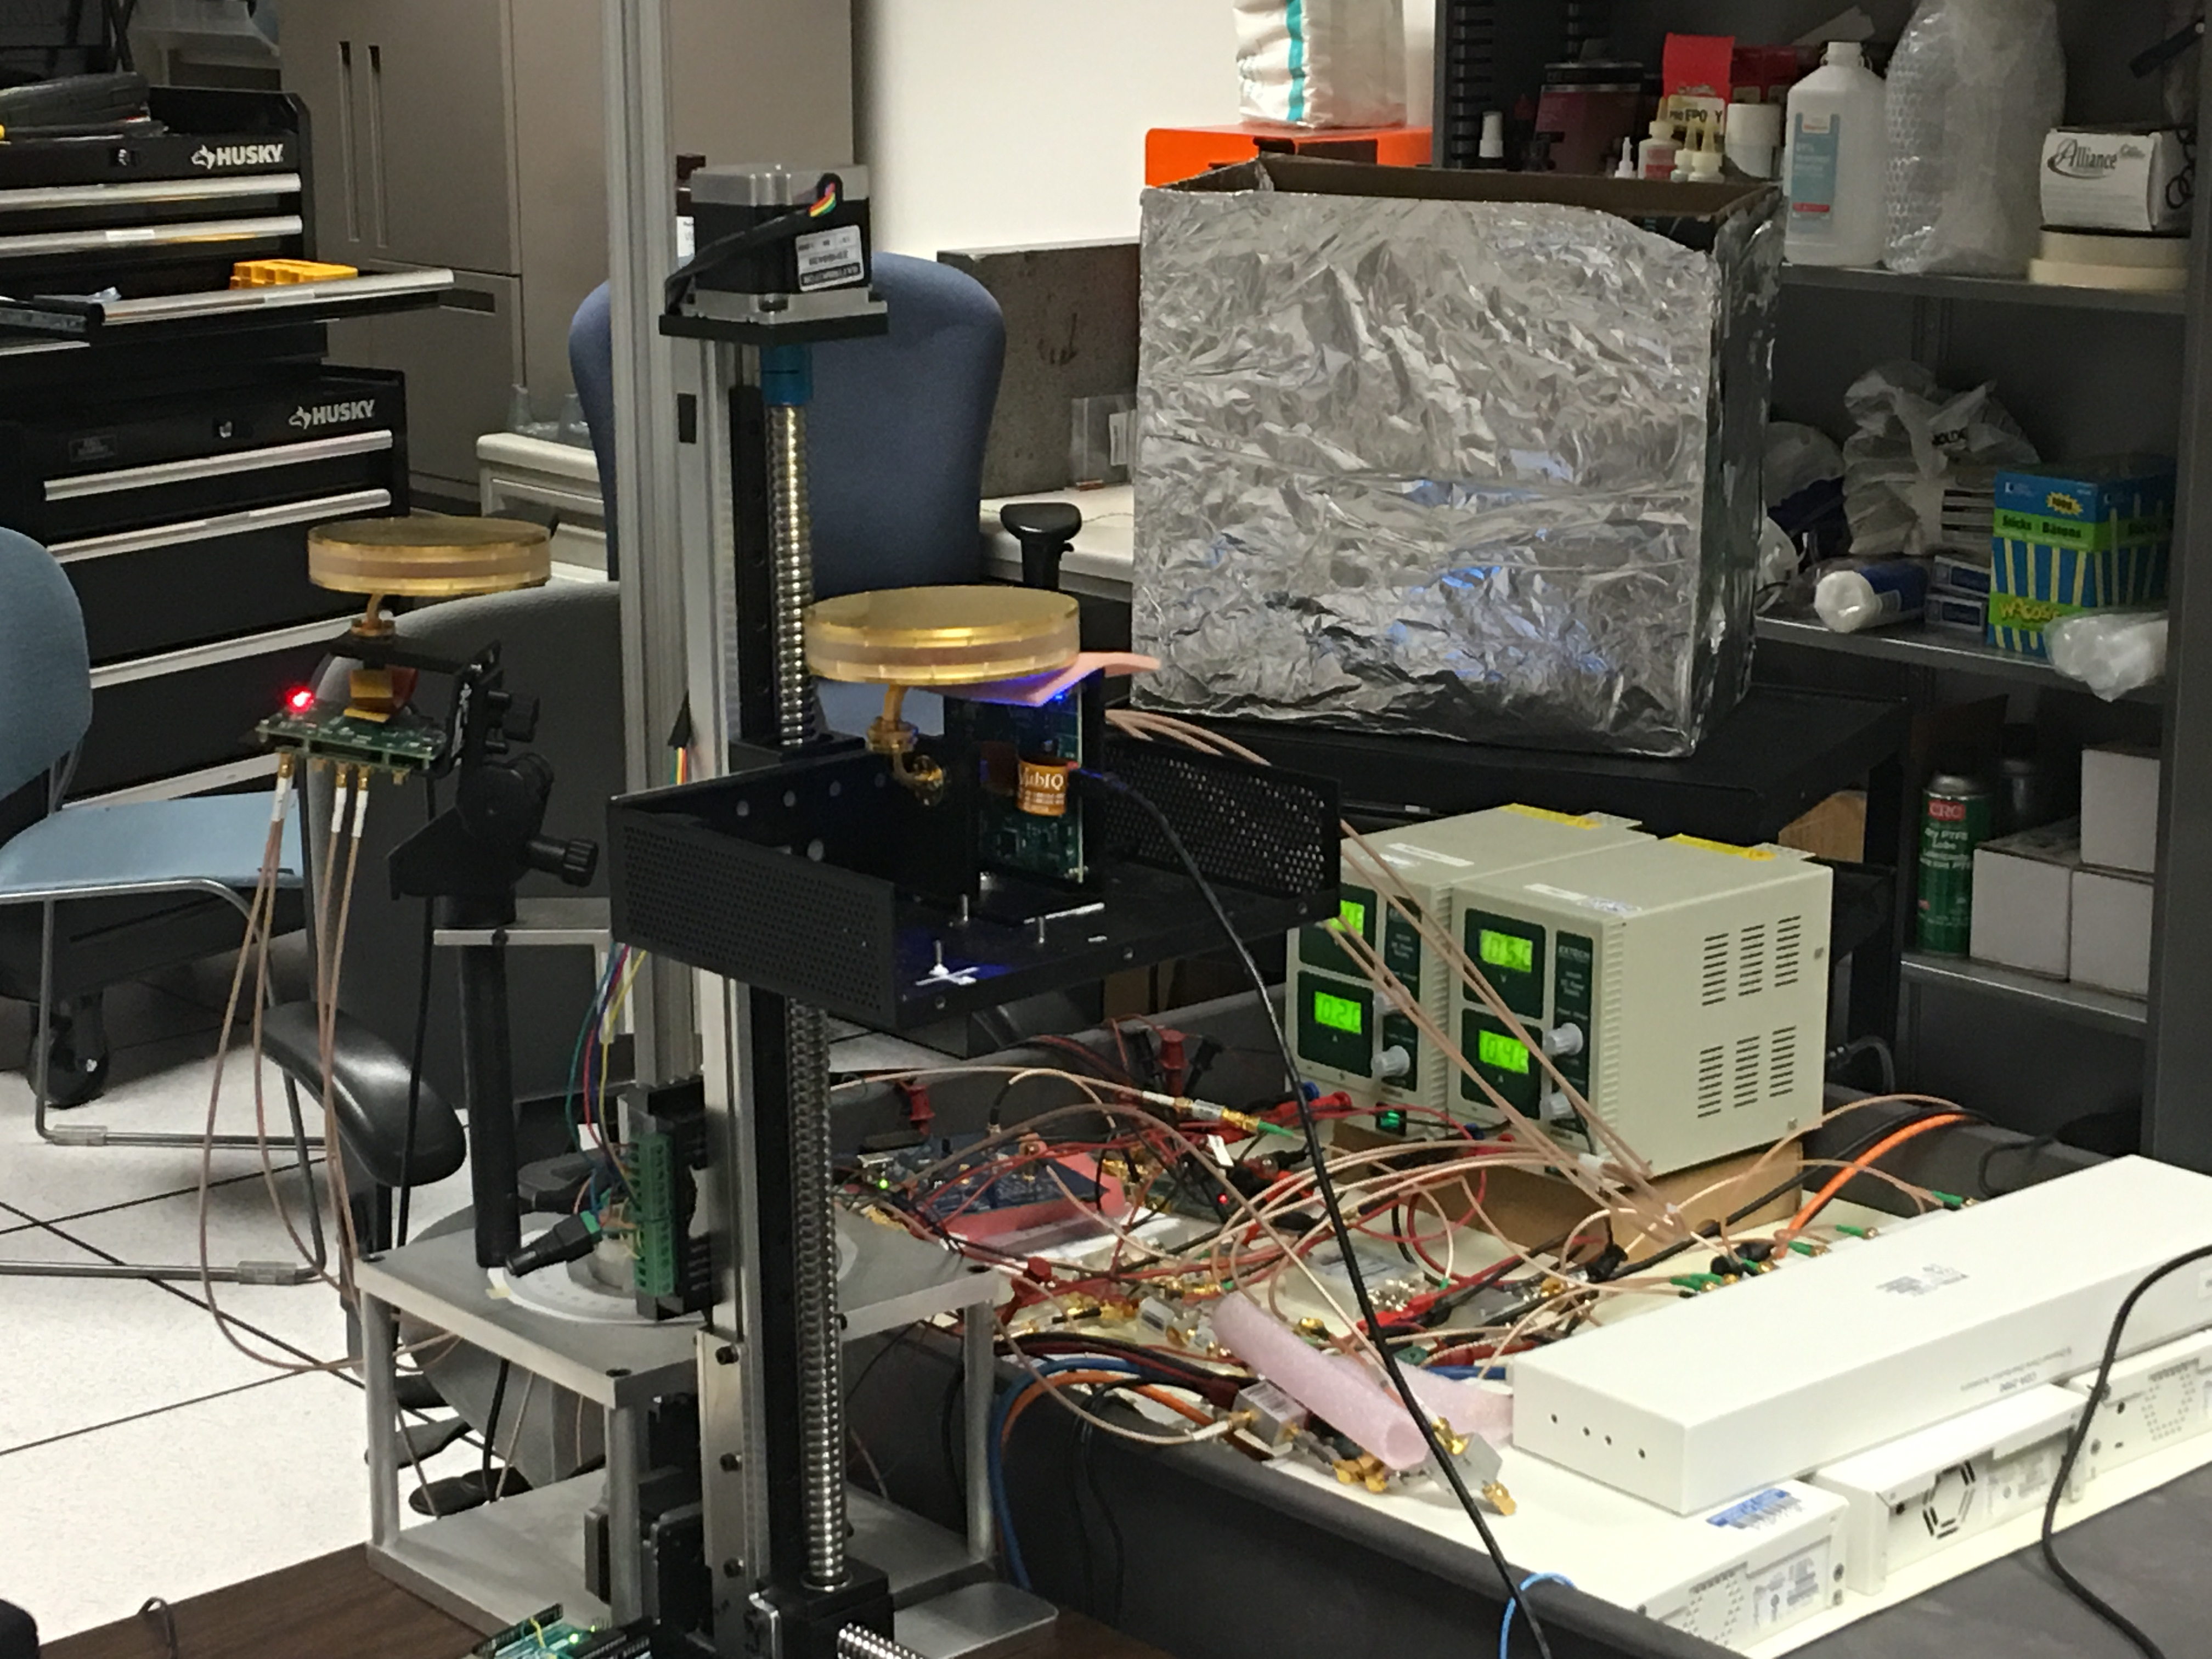
\includegraphics[width=8cm,height=6cm]{./figure/experiment_setup.jpg}
\caption{Custom-built 60 GHz mmWave radar imaging system}
\end{figure}

\fi
	% Sohrab

%section
\section{Discussion and Conclusion}
\textcolor{red}{
Analyze the results, summarize the findings and point out possible future directions
}

{\small
\bibliographystyle{ieee}
\bibliography{egbib}
}



\end{document}
